\documentclass{beamer} %

%%%BASICS
\usepackage[utf8]{inputenc}
\usepackage[T1]{fontenc}
\usepackage{lmodern}
\usepackage{amsmath, amssymb}
\usepackage{semantic}
\usepackage{appendix}
\usepackage{babel}
\usepackage{xcolor} % to access the named colour LightGray
\usepackage{minted}
\usepackage{pgfplots} % package used to implement the plot

%%%START THEME SETTINGS
\usetheme{CambridgeUS}
\usecolortheme{beaver} % seahorse, dolphin, default, beaver
\usefonttheme{professionalfonts}
\useinnertheme{rectangles}
% \useoutertheme{infolines}

\definecolor{lred}{RGB}{255,245,245}
\definecolor{mred}{RGB}{200,40,40}
\definecolor{dred}{RGB}{170,0,0}

\setbeamercolor{block title}{fg=white,bg=dred}
\setbeamercolor{block body}{bg=lred}
\setbeamercolor{section in toc}{fg=alerted text.fg}
\setbeamercolor{section in toc shaded}{bg=structure!20, fg=mred}
\setbeamercolor{section number projected}{fg=mred, bg=mred,fg=white}
\setbeamercolor{subsection number projected}{fg=mred, bg=mred,fg=white}
\setbeamertemplate{itemize item}{\color{mred}$\blacksquare$}
\setbeamertemplate{itemize item item}{\color{mred}$\blacksquare$}
% \setbeamertemplate{enumerate item}{\color{mred}$\blacktriangleright$}
\setbeamertemplate{enumerate item}{\color{mred}$\bullet$}

\setbeamercovered{transparent}
%%%END THEME SETTINGS


%------------------------------------------------------
\title[Mini-Lustre $\mapsto$ LLVM]{Compilation de Mini-Lustre vers LLVM}
\institute[UPSaclay]{Université Paris-Saclay}
\author{Lemaire \& Patault}
\date{\today}
%------------------------------------------------------

\newcommand{\ocaml}[1]{\mintinline{ocaml}{#1}}

\newcommand{\angArr}{
    \rotatebox[origin=c]{180}{$\Lsh$}
}

\pgfplotsset{width=6.5cm, compat=1.17}

\begin{document}
%------------------------------------------------------

\begin{frame}
    \titlepage
\end{frame}

%%%%%%%%%%%%%%%%%%%%%%%%%%%%%%%%%%%%%%%%%%%%%%%%%%%%%%%%%%%%%%%%%%%%%%%%%%%%%%%%%%%%%%%%%%%%%%%%%%%
\section{Introduction}
%%%%%%%%%%%%%%%%%%%%%%%%%%%%%%%%%%%%%%%%%%%%%%%%%%%%%%%%%%%%%%%%%%%%%%%%%%%%%%%%%%%%%%%%%%%%%%%%%%%

\begin{frame}
    \tableofcontents[currentsection]
\end{frame}

\begin{frame}[fragile]{Présentation Générale}
            \vfill
    \begin{itemize}
        \item LLVM := Low Level Virtual Machine

        \vfill\item LLMV IR := langage intermédiare que l'on utilise

        \vfill\item Interface C++ et bindings OCaml
    \end{itemize}
            \vfill
\end{frame}

%%%%%%%%%%%%%%%%%%%%%%%%%%%%%%%%%%%%%%%%%%%%%%%%%%%%%%%%%%%%%%%%%%%%%%%%%%%%%%%%%%%%%%%%%%%%%%%%%%%
\subsection{Présentation LLVM}
%%%%%%%%%%%%%%%%%%%%%%%%%%%%%%%%%%%%%%%%%%%%%%%%%%%%%%%%%%%%%%%%%%%%%%%%%%%%%%%%%%%%%%%%%%%%%%%%%%%

\begin{frame}{Pourquoi compiler vers LLVM ?}
    \vfill
    \begin{itemize}
        \item “Assembleur de haut niveau”
        \begin{enumerate}
            \item Typage
            \item Pointeurs
            \item Vecteurs
            \item Tableaux
            \item Structures
            \item Fonctions
            \item ...
        \end{enumerate}
    \vfill \item Bindings simples d'utilisation
    \vfill \item Compilateur optimisant vers toutes les architectures
    \end{itemize}
    \vfill
\end{frame}

%%%%%%%%%%%%%%%%%%%%%%%%%%%%%%%%%%%%%%%%%%%%%%%%%%%%%%%%%%%%%%%%%%%%%%%%%%%%%%%%%%%%%%%%%%%%%%%%%%%
\subsection{Utilisation LLVM}
%%%%%%%%%%%%%%%%%%%%%%%%%%%%%%%%%%%%%%%%%%%%%%%%%%%%%%%%%%%%%%%%%%%%%%%%%%%%%%%%%%%%%%%%%%%%%%%%%%%

\begin{frame}{Schéma de compilation simplifié}
    \begin{overprint}
    \onslide<1>
        \begin{figure}
            \centering
            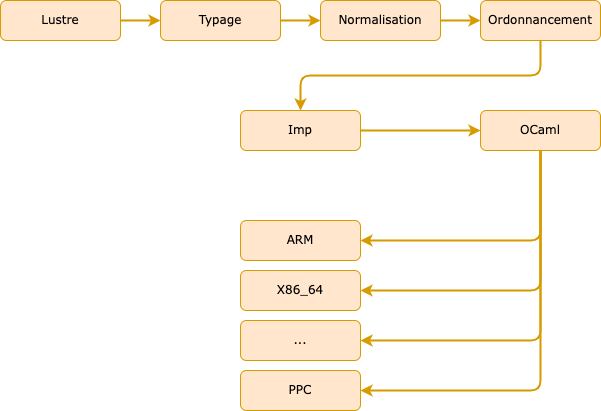
\includegraphics[width=0.8\textwidth]{imgs/compilation0.png}
        \end{figure}
    \onslide<2->
        \begin{figure}
            \centering
            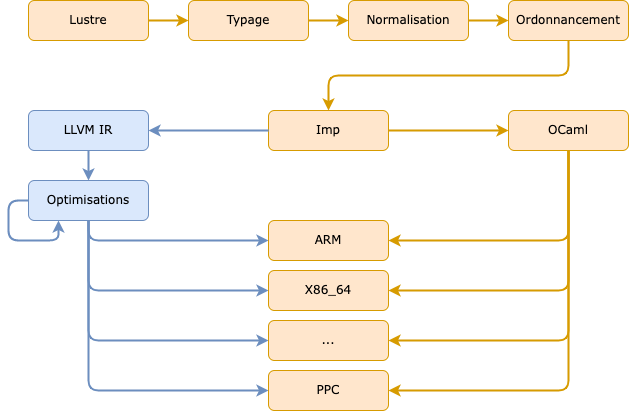
\includegraphics[width=0.82\textwidth]{imgs/compilation1.png}
        \end{figure}
    \end{overprint}

\end{frame}


\begin{frame}[fragile]{En pratique}
    \vfill
    \begin{itemize}
        \vfill\item Interface C++ et bindings OCaml
        \begin{minted}[baselinestretch=1.2,fontsize=\footnotesize]{ocaml}
    let main = Llvm.declare_function "main" i32 in
    let o = Llvm.build_alloca llvm_typ "o" llvm_builder in
    let one = Llvm.const_int i32_ty 1 in
    let store = Llvm.build_store o one llvm_builder in
    ...
        \end{minted}

        \vfill\item
        Génération du code LLVM IR (fichiers .ll)
        \begin{minted}[baselinestretch=1.2,fontsize=\footnotesize]{llvm}
    declare i32 @main() #0 {
      entry:
        %o = alloca i32, align 4
        store i32 1, i32* %o, align 4
        ...
    }
        \end{minted}
    \end{itemize}
\vfill
\end{frame}

%%%%%%%%%%%%%%%%%%%%%%%%%%%%%%%%%%%%%%%%%%%%%%%%%%%%%%%%%%%%%%%%%%%%%%%%%%%%%%%%%%%%%%%%%%%%%%%%%%%
\section{Travail Réalisé}
%%%%%%%%%%%%%%%%%%%%%%%%%%%%%%%%%%%%%%%%%%%%%%%%%%%%%%%%%%%%%%%%%%%%%%%%%%%%%%%%%%%%%%%%%%%%%%%%%%%

\begin{frame}
    \tableofcontents[currentsection]
\end{frame}

%%%%%%%%%%%%%%%%%%%%%%%%%%%%%%%%%%%%%%%%%%%%%%%%%%%%%%%%%%%%%%%%%%%%%%%%%%%%%%%%%%%%%%%%%%%%%%%%%%%
\subsection{Dans le dur}
%%%%%%%%%%%%%%%%%%%%%%%%%%%%%%%%%%%%%%%%%%%%%%%%%%%%%%%%%%%%%%%%%%%%%%%%%%%%%%%%%%%%%%%%%%%%%%%%%%%

\begin{frame}[fragile]{Exemple de transformation}
    \begin{columns}
    \begin{column}{0.25\textwidth}
  \begin{minted}[baselinestretch=1.2,fontsize=\footnotesize]{ocaml}
node f(x:int)
returns (o:int);
let
 o = 1;
tel
   \end{minted}
    \end{column}
    \begin{column}{0.05\textwidth}
        $\mapsto$
    \end{column}
    \begin{column}{0.70\textwidth}  %%<--- here
  \begin{minted}[baselinestretch=1.2,fontsize=\footnotesize]{llvm}
define i64 @f_1_step(i32 x) {
  %o = alloca i32, align 4
  store i32 1, i32* %o, align 4
  %0 = alloca %ret_f_1_step, align 8
  %1 = getelementptr inbounds ret_f_1_step,
            %ret_f_1_step* %0, i32 0, i32 0
  %2 = load i32, i32* %o, align 4
  store i32 %2, i32* %1, align 4
  %3 = bitcast %ret_f_1_step* %0 to i64*
  %4 = load i64, i64* %3, align 4
  ret i64 %4
}
   \end{minted}
    \end{column}
    \end{columns}
\end{frame}

%%%%%%%%%%%%%%%%%%%%%%%%%%%%%%%%%%%%%%%%%%%%%%%%%%%%%%%%%%%%%%%%%%%%%%%%%%%%%%%%%%%%%%%%%%%%%%%%%%%
\subsection{Benchmarks}
%%%%%%%%%%%%%%%%%%%%%%%%%%%%%%%%%%%%%%%%%%%%%%%%%%%%%%%%%%%%%%%%%%%%%%%%%%%%%%%%%%%%%%%%%%%%%%%%%%%


\begin{frame}{Performances}
    \begin{table}[h]
        \begin{center}
            \begin{tabular}{|r|c|c|c|}\hline
                                & simple.mls ($10^7$) & simple.mls ($10^8$) & todo.mls \\ \hline\hline
                          LLVM  & 13.84s             & 140.70s            & todo     \\ \hline
                          OCaml & 16.29s             & 185.49s            & todo     \\ \hline
                          % Lustre compiler & 11s       & 9s        & 19s       \\ \hline
            \end{tabular}
            \caption{Table des performances comparées en fonction du langage cible}
        \end{center}
    \end{table}
\end{frame}

% \begin{frame}{Performances}
%     \begin{tikzpicture}
%         \begin{axis}
%             [
%             ybar, % ybar command displays the graph in horizontal form, while the xbar command displays the graph in vertical form.
%             enlargelimits=0.15,% these limits are used to shrink or expand the graph. The lesser the limit, the higher the graph will expand or grow. The greater the limit, the more graph will shrink.
%             legend style={at={(0.4,-0.25)}, % these are the measures of the bottom row containing surplus (wheat, Tea, rice), where -0.25 is the gap between the bottom row and the graph.
%             anchor=north,legend columns=-1},
%             % here, north is the position of the bottom legend row. You can specify the east, west, or south direction to shift the location.
%             symbolic x coords={Ex1, Ex2, Ex3},
%             xtick=data,
%             nodes near coords,
%             nodes near coords align={vertical},
%             ]
%             \addplot coordinates {(Ex1, 75) (Ex2, 78) (Ex3, 80)}; % these are the measures of a particular bar graph. The tick marks of the y-axis will be adjusted automatically according to the data values entered in the coordinates.
%             \addplot coordinates {(Ex1, 70) (Ex2, 63) (Ex3, 68)};
%             \legend{LLVM, OCaml}

%         \end{axis}
%     \end{tikzpicture}
% \end{frame}

%%%%%%%%%%%%%%%%%%%%%%%%%%%%%%%%%%%%%%%%%%%%%%%%%%%%%%%%%%%%%%%%%%%%%%%%%%%%%%%%%%%%%%%%%%%%%%%%%%%
\subsection{Démonstration}
%%%%%%%%%%%%%%%%%%%%%%%%%%%%%%%%%%%%%%%%%%%%%%%%%%%%%%%%%%%%%%%%%%%%%%%%%%%%%%%%%%%%%%%%%%%%%%%%%%%

\begin{frame}{Démonstration}
    En direct
\end{frame}


\end{document}
